% a little more material could be added from IESA 2017-04-12


% 2019-03-27

\documentclass[10pt]{article}
\usepackage[T1]{fontenc}
\usepackage{amssymb}
\usepackage{amsmath}
\usepackage{graphicx}
% \begin{figure}[h]
% \centering
% \includegraphics[width=6.5in]{folder/photo.png}
% \caption{}
% \label{}
% \end{figure}



\usepackage{tikz}
\usetikzlibrary{arrows}
\usepackage{subfigure}
\usepackage{stackrel}
\usepackage{blindtext}

\usepackage{biblatex}
\addbibresource{library.bib}

\oddsidemargin=0.15in
\evensidemargin=0.15in
\topmargin=-.5in
\textheight=9in
\textwidth=6.25in

\usepackage[colorlinks=true,breaklinks,pdfpagemode=none,linkcolor=blue,citecolor=blue]{hyperref}

\usepackage{enumerate}
% \vspace{-6pt}
% \begin{itemize}
%     \setlength{\itemsep}{0pt}%
%     \setlength{\parskip}{0pt}%
%     \item Item 1
%     \item Item 2
%         \begin{itemize}
%             \setlength{\itemsep}{0pt}%
%             \setlength{\parskip}{0pt}%
%             \item Sublist Item 1
%             \item Sublist Item 2
%         \end{itemize}
%         \item Item 3
% \end{itemize}
% \vspace{-6pt}


\usepackage{enumitem}
\setlist{itemsep=0mm}

%\usepackage{description}

\usepackage{amsmath,amsfonts,amssymb,bm}


\begin{document}

   \noindent
   \begin{center}

   \hrulefill
   
   \vspace{5pt}
   
   \makebox[\textwidth]{ {\bf Energy Systems Analysis} \hfill  A.D. Smith 2019}
   \vspace{0pt}
   
   {\Large \hfill  Lecture 27.  
Uncertainty Analysis (UA) for Models
}
   \vspace{5pt}
   
  
   \hrulefill
   \end{center}
   
   {\color{darkgray}{\center{ \small{      ``Uncertainty is not a weakness. Understanding uncertainty is a strength, and a key part of using any model \ldots''
\\%[3pt]
\rightline{{\rm --- Gettelman and Rood \cite{Gettelman2016-my}}}}}}}


\section{What is uncertainty analysis?}
Let's start with why we might look to analyze uncertainty. Gettelman and Rood have a thorough definition of uncertainty itself, and Coleman and Steele have a very simple definition for uncertainty analysis (UA).

\begin{description}
\item [\textbf{uncertainty}] ``the noncorrectable or unknown part of the inaccuracy of an instrument, system, or model. Uncertainty represents the limit of measurement (or forecast) precision.''\cite{Gettelman2016-my}
\item [\textbf{uncertainty analysis}] ``the analysis of the uncertainties in experimental measurements and in experimental and simulation results.''\cite{Coleman2009-wb}
\end{description}

\medskip
            \begin{figure}[h]
            \centering
            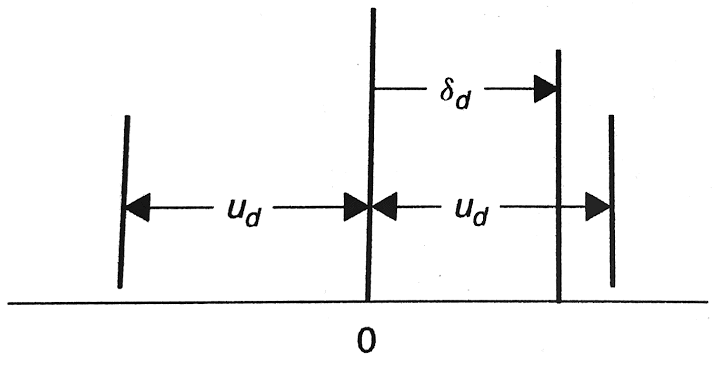
\includegraphics[width=6cm]{extras27/u}
            \caption{An uncertainty \textit{u} defines an interval that is estimated to contain the actual value of an error of unknown sign and magnitude. \cite{Coleman2009-wb}}
            \label{coleman1.3}
            \end{figure}
\bigskip



\subsection{Why perform UA?}
% Saltelli 
% \cite{Saltelli2009-tz} states that the goal of sensitivity analysis is to ``to apportion the variation in the output to the different sources of variation in the system.''\\

When performing an uncertainty analysis, we are asking these kinds of questions:

\begin{itemize}
\item How much of a \textit{big deal} is it if I'm not too confident in something going into my model?
\item What is the effect of \textit{stochastic variations} in some input(s) on the output(s) of the model?
\item  What is the effect of having a \textit{range of potential values} or a particular \textit{distribution of potential values} in some input(s) on the output(s) of the model?
\end{itemize}

So uncertainty analysis is a deeper look at what we don't know and how it impacts us. These questions go hand-in-hand with sensitivity analysis.

\section{Sources of uncertainty}

Recognizing that uncertainty describes things we can't correct or know completely, it is easy to identify many sources of uncertainty when you apply a critical eye toward modeling problems and measurements taken from energy systems. Imagine that in Fig. \ref{coleman1.4} you have a thermocouple taking a temperature measurement. What are five things that could be causing your measurement to stray from the `true' value?

Because computational models depend on some form of experimental measurements or empirical data (or at least \href{https://en.wikipedia.org/wiki/Verification_and_validation_of_computer_simulation_models}{they should!}), the modeler has to deal with uncertainty from experimental data as well as uncertainty associated with the computer simulation itself. Considering how uncertainty compounds throughout the data gathering-modeling-simulation process is called \textbf{uncertainty propagation}, and is illustrated in Fig. \ref{coleman3.4}.

\medskip
            \begin{figure}[h]
            \centering
            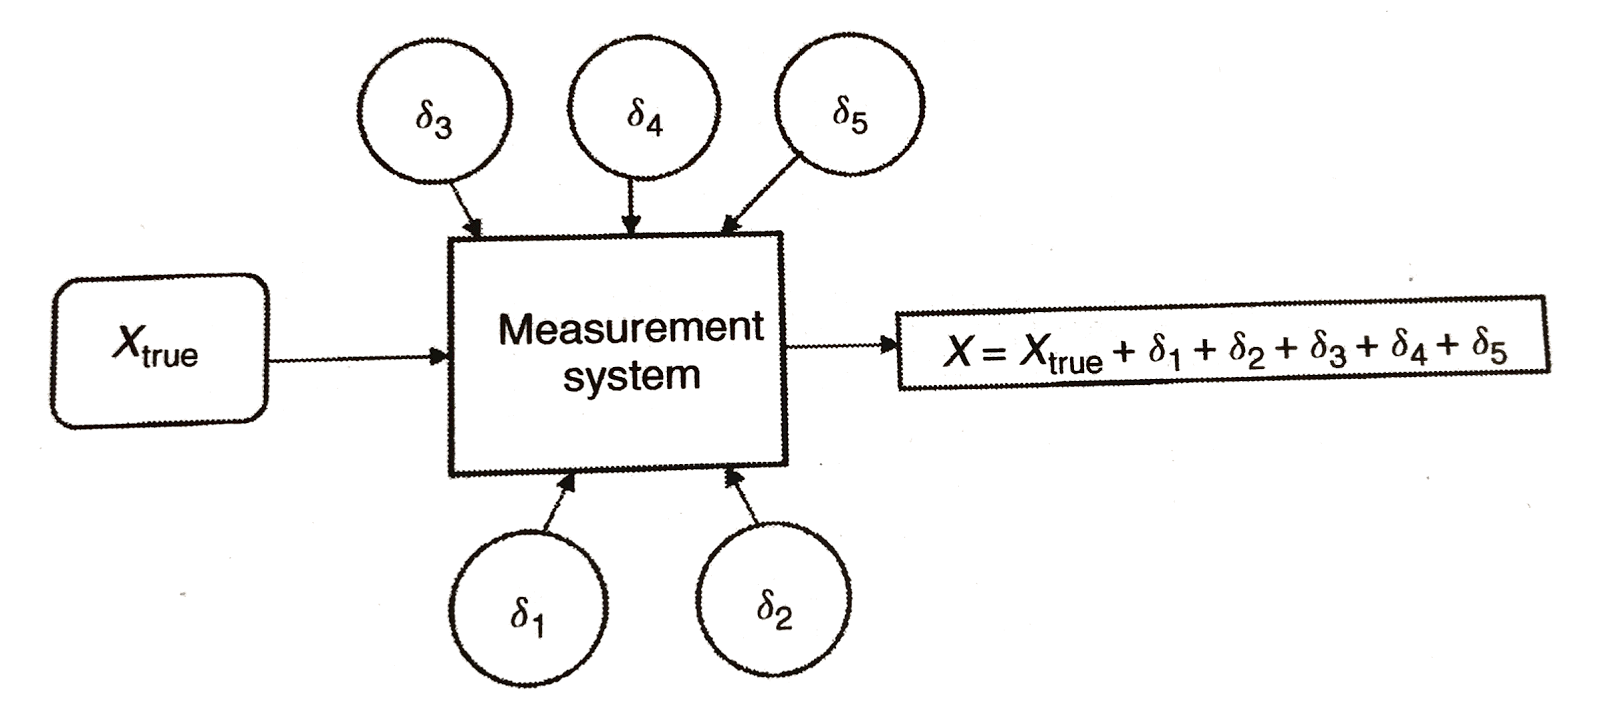
\includegraphics[width=8cm]{extras27/meas}
            \caption{Measurement of a variable influenced by five error sources. \cite{Coleman2009-wb}}
            \label{coleman1.4}
            \end{figure}
\bigskip

\medskip
            \begin{figure}[h]
            \centering
            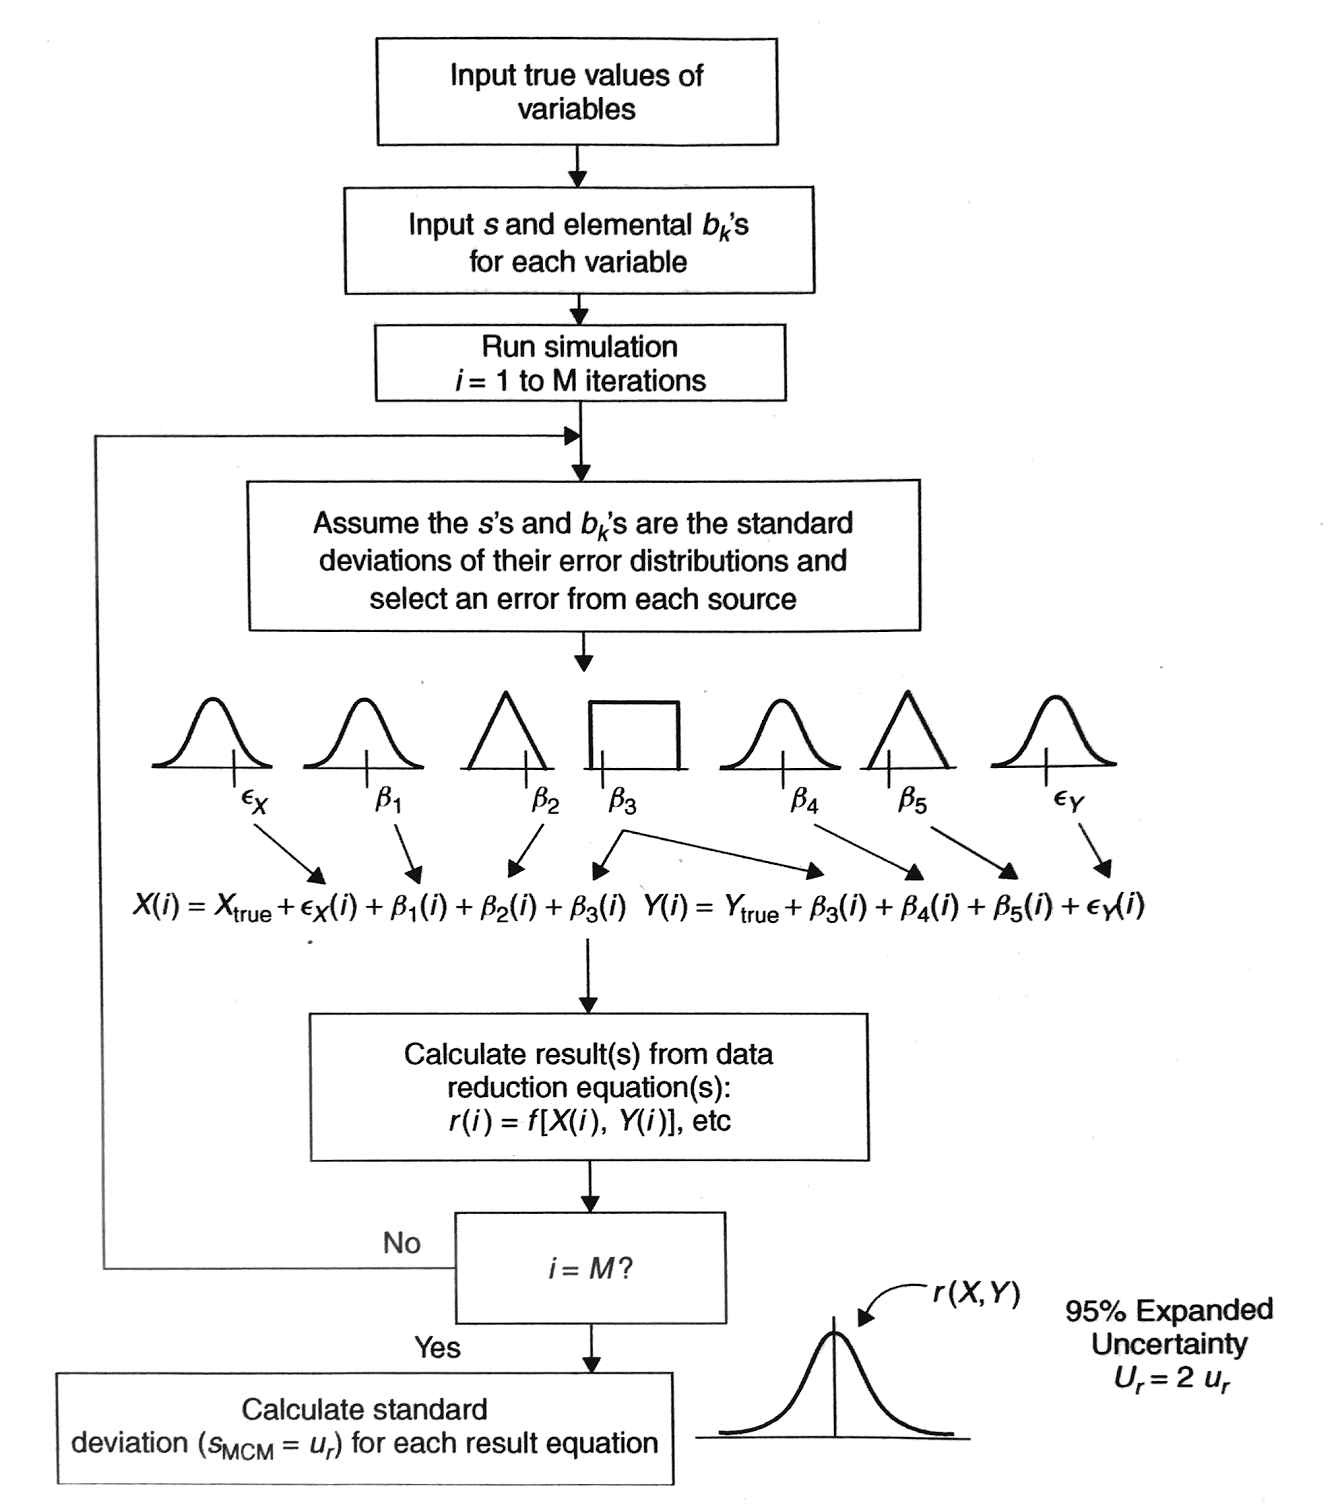
\includegraphics[width=11cm]{extras27/schem}
            \caption{Schematic of Monte Carlo Method for uncertainty propagation when random standard uncertainties for individual variables are used. \cite{Coleman2009-wb}}
            \label{coleman3.4}
            \end{figure}
\bigskip

We may be concerned with uncertainty in:
\begin{itemize}
\item Empirical data used within the model, or to validate the model
\item Calculated data
\item The structure of the model itself
\item Model parameters
\end{itemize}

\section{Uncertainty considerations in the modeling process}

The following list is adapted from Coleman and Steele \cite{Coleman2009-wb}, who provide these questions to be considered as part of designing your experimental approach. However, considering the computer simulation to be a kind of numerical `experiment,' they apply quite well.

\begin{enumerate}
    \item What question are we trying to answer?
    \item How accurately do we need to know the answer? (How will we use the answer?)
    \item What physical principles are involved? (What are the governing equations?)
    \item What model or set of simulation techniques might provide the answer?\\
    \ldots
    \item Can the requirements be satisfied within the budget and time constraints (including computational time)?
    \item What techniques should be used to analyze the data?
    \item What is the most effective way to present the data?
    \item What unanticipated questions are raised by the data? (Should we revisit prior steps or redesign our modeling process?)
    \item How can we best report the data and results?    
\end{enumerate}
    


\section{Bayesian model averaging for uncertainty estimation}

In classical statistics, models are created similarly to the flowchart in Fig. \ref{coleman3.4}. The analyst knows or assumes some distributions for the variables and proceeds from there. You should recognize $ \beta_1 $ as a normal distribution and $\beta_3$ as a uniform distribution. $\beta_2$ is another simple distribution called a triangular distribution, which is pretty self-explanatory.

Bayesian statistical approaches turn this usual pattern on its head. Pfeiffer describes it this way: ``Since the population mean is a quantity about which there is uncertainty, it is modeled as a random variable whose value is to be determined by experiment. In this view, the population distribution is conceived as randomly selected from a class of such distributions.'' \cite{Pfeiffer2009-prob}. Here, the population mean represents the `true' value and the experiment can be a computational simulation. 

If you've taken a statistics course, you may remember the 'chain rule' provided by Bayes that describes how likely it is for something to happen \textit{given that you know the likelihood of something else that is related to the event you are interested in}. Christian and Griffiths \cite{Christian2016-ug} point out that Bayes' Rule ``makes it possible to \textit{reverse-engineer} all kinds of prior distributions, even ones about which it's harder to get authoritative real-world data." It follows, then, that "the richer the prior information we bring to Bayes' rule, the more useful predictions we can get out of it'' \cite{Christian2016-ug}. This is true for practically any modeling technique you will use: If `rich' data means it is more representative of the system/process you are trying to model, then additional data and higher quality data will improve your predictive accuracy. You may remember that the representativeness of the data set was a key concern for creating machine learning-based models.

Bayesian model averaging is simply a way to implement this statistical knowledge for the benefit of our modeling efforts. Monte Carlo (randomized sampling) methods are frequently used, and Saltelli et al. \cite{Saltelli2004-ga} describes a case study using the Generalized Likelihood Uncertainty Estimation (GLUE) approach, which is a simplified way to implement Bayesian inference using a weighting function. They also caution that ``It is necessary that the sample generated for the Bayesian analysis is also designed for the computation of variance-based sensitivity indices," \cite{Saltelli2004-ga} which is important when performing a combined GSA-UA analysis of a model. \\

\noindent{}
Key ideas on Bayesian Model Averaging  \cite{Saltelli2004-ga}:
\begin{itemize}
\item Attempts to take into account all possible sources of uncertainty
\item Bayesian statistical methods account for the likelihood of events given other known distributions or likelihoods
\item  GLUE \cite{Saltelli2004-ga, Blasone2008-av} is just one method of implementing this.
\end{itemize}

\medskip

\noindent{}
Possibilities for using GSA in Bayesian uncertainty estimation \cite{Saltelli2004-ga}:

\begin{itemize}
\item Model output itself
\item \textbf{Likelihood} \hspace{0.25cm} ``a function that quantifies how well that
particular parameter combination (or model) simulates the system'' \cite{Blasone2008-av}
\end{itemize}

%likelihood meaning, "How likely is this over a certain parameter space?"
\noindent
Here is a free book (web version) from Green Tea Press that is a great resource for learning more about Bayesian analysis (particularly if you already use Python):\\

\href{http://greenteapress.com/wp/think-bayes/}{Think Bayes} \cite{Downey2013-ma}\\


We may use GSA and Bayesian uncertainty estimation together to gain better information about which factors are most important, how complex the model and factor interactions is/are, and which factors are involved in those interactions and in the model outcome.

% license
\bigskip

\noindent
\texttt{\footnotesize RESTRICTED PUBLIC LICENSE --- READ BEFORE SHARING. This is a draft version made available by Amanda D. Smith under a Creative Commons Attribution-NonCommercial-ShareAlike license. 
\href{https://creativecommons.org/licenses/by-nc-sa/4.0/}{CC BY-NC-SA 4.0}}

% references

\printbibliography

\end{document}